\section{Guided Model Selection}
\label{sec:guidedModelSelection}

Our second approach is to guide a human in the loop choosing the best model. We still recommend a top model that can be automatically chosen, but we have no guarantee it will perform best. Hence, we called this approach \emph{Guided}. The idea is to split forecasting tasks and its timeseries data into groups. We then evaluate several models against these grouped timeseries and again record the scores. When a user wants to create a new forecast and needs to select a model, we look at the group this forecasting task and the timeseries belong to and lookup the recommended models for this group.

\subsection{Groups}

We create groups based on forecasting task parameters and features extracted from the timeseries $T$ itself. The first variable is the user defined forecast horizon $fh$. The other variables are determined by the timeseries. We use frequency $freq$, window length $len(T)$, principal seasonal period $sp$ and if the data is strictly positive. We regard frequency as one of the base frequencies minute, hour, day, month and year. Each base frequency can have multiple resolutions, e.g., a data point every 5 minutes. The exact configurations we used are shown in table \ref{tab:groupConfigs}. Additionally, to the criteria shown there, we separate timeseries which are strictly positive or not, as this can restrict some models from working well (or their hyper-parameters).

We then create all possible combinations of these configuration parameters, which results in 580 different groups. This includes invalid configurations, e.g., the seasonal period is 365 days but the window length is only 7 days. We drop invalid combinations according to the following rules:

\begin{itemize}
    \setlength\itemsep{.1cm}
    \item Horizon is smaller than resolution
    \item Horizon is larger than the start interval of the window by a factor of 2
    \item Seasonality is larger than the start interval of the window by a factor of 4
\end{itemize}



\begin{table*}
  \fontsize{8.5pt}{8.5pt}\selectfont
  \caption{Group Configurations}
  \centering
  \begin{tabular}{p{3cm}|p{11.2cm}}
     
     Frequency & Parameters\\
     
     \hline
     \vspace{.01cm}
     Minute $m$ & 
     \vspace{-.5cm}
     \begin{itemize}
         \setlength\itemsep{0cm}
         \item Window Length: [0s, 10m), [10m, 3h), [3h, 7d), [7d, 28d)
         \item Resolution: 1m, 5m
         \item Seasonality: none, 1h, 24h
         \item Horizon: 1 step, 1h, 24h
     \end{itemize}  \\
     \hline
     
     \vspace{.01cm}
     Hour $h$ & 
     \vspace{-.5cm}
     \begin{itemize}
         \setlength\itemsep{0cm}
         \item Window Length: [0h, 24h), [24h, 7d), [7d, 28d), [28d, 5y)
         \item Resolution: 1
         \item Seasonality: none, 1d, 7d
         \item Horizon: 1 step, 12h, 24h, 7d
     \end{itemize}  \\
     \hline
     
     \vspace{.01cm}
     Day $d$ & 
     \vspace{-.5cm}
     \begin{itemize}
         \setlength\itemsep{0cm}
         \item Window Length: [0d, 56d), [56d, 180d), [180d, 480d), [480d, 4y), [4y, 100y)
         \item Resolution: 1d, 7d
         \item Seasonality: none, 7d, 365d
         \item Horizon: 1 step, 28d, 60d, 365d
     \end{itemize}  \\
     \hline
     
     \vspace{.01cm}
     Month $M$ & 
     \vspace{-.5cm}
     \begin{itemize}
         \setlength\itemsep{0cm}
         \item Window Length: [0M, 6M), [6M, 2y), [2y, 10y), [10y, 200y)
         \item Resolution: 1M
         \item Seasonality: none, 12M
         \item Horizon: 1 step, 6M, 12M, 24M, 48M
     \end{itemize}  \\
     \hline
     
     \vspace{.01cm}
     Year $y$ & 
     \vspace{-.5cm}
     \begin{itemize}
         \setlength\itemsep{0cm}
         \item Window Length: [0y, 10y), [10y, 2000y)
         \item Resolution: 1y
         \item Seasonality: none
         \item Horizon: 1 step, 2y, 5y, 10y, 20y
     \end{itemize}  \\
     \hline
  \end{tabular}
  \label{tab:groupConfigs}
\end{table*}


This gives us a list of slightly over 300 group configurations. The list of discriminative features has defined based on the insights generated by the M4 competition \cite{M4} and \cite{sktime}, that simple models can achieve almost unbeatable results in lower resolution datasets. One insight was that the baseline forecasts for the hourly data of the M4 competition was harder to beat than the daily timeseries. To also split by window length, seasonality and horizon, we hypothesize that some models that will perform worse or better depending on whether there is a lot of data available (window length), if seasonality is present and if the horizon is short or long.

\subsection{Datasets}

The next step is to find datasets which can be grouped so every group has a minimal amount of timeseries for models to be evaluated against. Luckily, we do not have to find 296 different datasets as we can ignore the forecast horizon. We can also resample low resolution timeseries to receive a higher resolution and base frequency. For the window length we can use the same series multiple times by cutting it of at the end interval of the window length. This means that the true factors making a timeseries not available for a group are seasonality, too few data points to satisfy window length and if the series is strictly positive or not.

To generate timeseries for each group we built a framework that implements a series of dataset sources, applies resampling and evaluates if the timeseries matches the group configuration requirements. Most features are easy to determine except the seasonal period.

In our scenario we used several built-in timeseries from sktime \cite{sktime} intended for forecasting (some sktime timeseries are intended for classification). These are good for daily, monthly and yearly groups. Another dataset we used is from Yahoo \cite{yahoo-dataset} and was intended to be used for anomaly detection research. It consists of about 350 timeseries with hourly resolution and 1,440 data points (60 days). We also created a wrapper for Our World In Data (OWID) COVID-19 timeseries \cite{OWID-COVID}. This data contains daily data since the beginning of the pandemic in 2020. By using the Kaggle competition datasets to forecast store sales \cite{STORE_SALES_COMPETITION} we enriched our corpus with long term daily data (3 years). For strictly positive daily data we used a dataset from a Network Traffic Analysis competition on Kaggle \cite{NETWORK_TRAFFIC_COMPETITION}. Finally, we also needed some strictly positive data in the minute frequency, which we found in climate data from the Max-Planck-Institute \cite{CLIMATE_DATASET}.

Our approach requires us to find diverse datasets that match our many groups. This can be a challenge, but we have found that it is possible for daily, monthly and yearly data. Acquiring hourly and minute resolution datasets can be a bigger challenge as those generally require more storage and open data publishers often do not expose these.

\subsection{Determining Seasonality}
% Move section somewhere else?

To split timeseries into different seasonal period groups, we need to automatically assign a seasonality as we do not have the capacity to label data ourselves. Each timeseries can contain multiple seasonalities which could be modeled using Fourier series. However, for our initial grouping we are interested in the principal seasonal period or the strongest one. 
Our approach is to compute the auto correlation function (ACF) with a maximum lag of the acceptable range for that frequency. We can then search for the highest peak with a peak finder algorithm. We require a minimal distance between peaks of 4, and minimal height difference of 0.1 and a prominence of 0.1. The prominence of a peak measures how much a peak stands out from the surrounding baseline of the signal and is defined as the vertical distance between the peak and its lowest contour line \cite{scipy}.


\begin{figure*}
\centerline{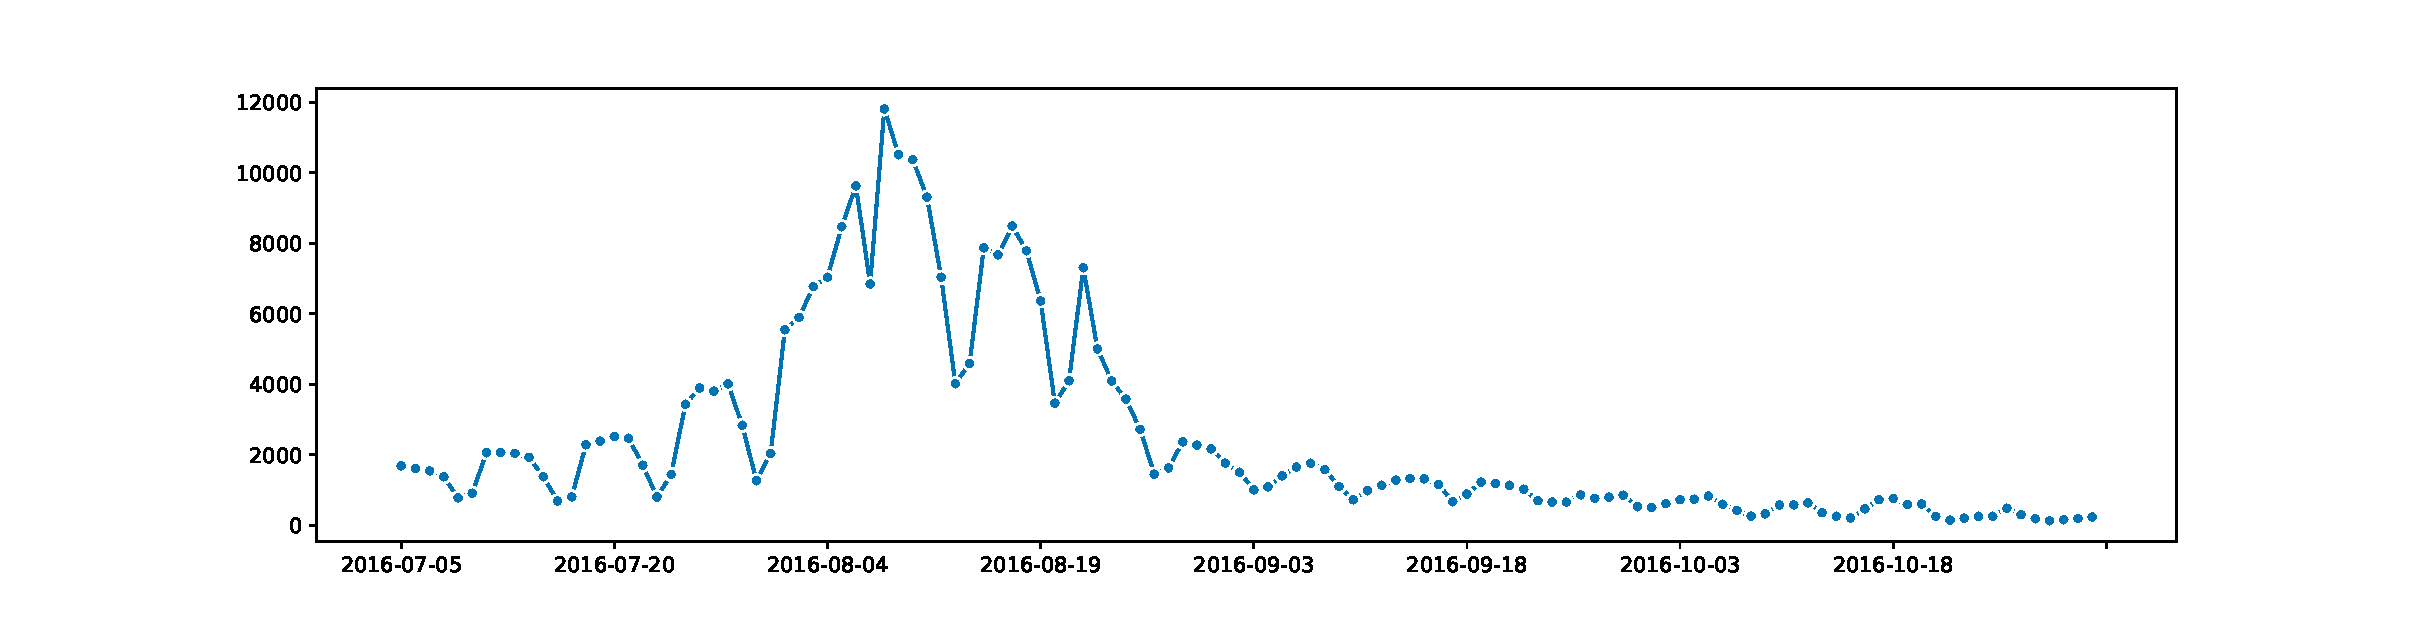
\includegraphics[scale=.4]{Figures/ts_example.eps}}
\caption{An example of a timeseries from the Web Traffic dataset that contains a weekly seasonality.}
\label{fig:ts_example}
\end{figure*}

\begin{figure*}
\centerline{\includegraphics[scale=.5]{Figures/acf.eps}}
\caption{Auto Correlation function plot of the timeseries in figure \ref{fig:ts_example}. The initial high number at 1 is the correlation of a point with the previous point, which we are not interested in. We can see a peak at 7 and repetitions at multiples of 7. Our algorithm determined a seasonal period of 7 for this example.}
\label{fig:acf}
\end{figure*}

This gives us a list of possible principal periods. Under certain circumstances the true period was not detected as a peak but it's multiples. To mitigate this, we check if the resulted peaks have a greatest common denominator larger than 1 and include this in our list. We then filter the found peaks for acceptable periods to remove false positives. This is removing abnormal but true seasonal periods, but it has shown that doing this greatly improves the overall usefulness of using seasonality as discriminative feature.

\newpage
Our defined acceptable seasonal periods are the following. The accepted period depends on the original frequency.

\begin{itemize}
    \item Minute: 5m, 1h, 12h, 1d,
    \item Hour: 24h, 7d
    \item Day: 7d, 365d
    \item Month: 12 months
    \item Year: no periods accepted
\end{itemize}

If the ACF peak algorithm finds a period outside of this list, we reject it.

\subsection{Evaluating Models}

To evaluate models against timeseries we are using the same method from \ref{sec:autoModelSelection} \emph{Auto Model Selection}, except we are now doing it for several dataset groups. We again collect error terms, time to fit and time to predict.

\subsection{Finding Model Recommendation}

We have collected the necessary data now to recommend a model for a new timeseries. The user has several metrics available to compare the models. However, if the number of timeseries is large, we still want to automatically select a model. Just choosing the model with the best accuracy is however not the best in terms of user satisfaction. We propose that the selection is done by first mapping the metric values to metric scores $0-1$. We then create a weighting average of the model metric scores and compose a model score. The user is in control of the weights and can thus influence the chosen model. Defining the weights can be done once and then applied to all timeseries model selections.
To map the metric value to a score we use log-normal curves with specified median $m$ and 10\textsuperscript{th} percentile $p_{10}$. The following equations define our mapping function with the location $\mu$ and the shape coefficient $\sigma$.

\begin{equation}
    \mu = \ln{m}
\end{equation}
\begin{equation}
    \sigma = \frac{\ln{p_{10}}}{\sqrt{2}*0.9061938024368232}
\end{equation}
\begin{equation}
    C(x)=\frac{1}{2}(1-E_{rf}(\frac{\ln{x} - \mu}{\sqrt{2}*\sigma}))
    \label{eq:logNormal}
\end{equation}

With the score on a log-normal curve we can create scoring buckets based on percentiles. In our case we chose $[1-0.9]$ for "model recommended", $(0.9-0.5]$ for "model acceptable" and $(0.5-0]$ for "model not recommended". An example is shown in figure \ref{fig:metric-mapping}. We set the curve control points by taking the 10\textsuperscript{th} and 50\textsuperscript{th} percentiles of the metric values of that metric for that group.

\begin{figure*}
\centerline{\includegraphics[scale=.33]{Figures/metric-mapping.pdf}}
\caption{The log-normal curve is mapping the metric value CPU time to a $0-1$ score. In this example we manually defined the control points $p10$ with 600ms and the median with 2000ms. The Point Of Diminishing Returns $podr$ is computed at 188ms. Meaning a model that achieves a time significantly below that is not going to get much reward for it. The upper green, middle orange and lower red section show the level of recommendation.}
\label{fig:metric-mapping}
\end{figure*}

Besides accuracy (RMSSE) and CPU time, we also assigned each model type an explainability category with scores. We used trivial ($1$), easy ($0.9$), medium ($0.8$) and hard ($0.5$) as categories. We did not find a way to determine explainability of a model other than using human perception of the model explanation itself.

Inspecting our model evaluation, we have discovered that certain model types are more consistently scoring low errors while others excel more sporadically. For example, we saw that the Poly Trend model was the best model of them all for several timeseries, but it was producing bad results for other timeseries. This is because its hyper parameter \emph{degree} is super sensitive. To change the model selection to tend towards more stable models we computed the RMSSE score for each forecast and took the standard deviation over all forecast errors. We then combine RMSSE with its standard deviation and map this to the accuracy score $0-1$ instead of just the mean.


\subsection{Results}

The resulting framework allows us to evaluate a series of models against a group of datasets and collect summaries. We can then use these summaries to decide which model we want to use by adjusting the weights for each selection variable accuracy, CPU time and explainability. With this approach we have to evaluate a range of models against a large and diverse set of datasets once, and then others can consume this in a quick, reliable and easy fashion. The decision which model to use for a new learning problem and timeseries can be computed within milliseconds, which accomplishes our initial goal. An example of a summary is shown in table \ref{tab:groupSummary}. As we will show in the evaluation section, this approach also generates final forecasts that outperform a generic model to rule them all while being fast to compute.

The quality of the summaries however depends on the diverse datasets that are used to build them. Having several hundred groups requires an assembly of datasets from different fields, different resolutions, different basic characteristics and different lengths. We were not able to find a lot of diverse timeseries data for our minute and hourly groups. But we can down sample data and shorten them to include the same source data in different groups. If we want to add more discriminative variables to split it into more groups, we will eventually fail to find data that matches these ever increasing criteria. However, we don't think that many more variables are necessary or should even be added.

In table \ref{tab:bestModelPerGroup} we show off how our proposed solution elected models solely based on accuracy per group. We find that certain models are working better in given groups than others. This proves that our used features of learning problem and timeseries create different spaces where different models work best.


\begin{table}
\fontsize{9pt}{12pt}\selectfont
\begin{tabular}{llllllr}
Freq. & $fh$ & $sp$ & Strictly pos. & Window & Winner & CPU Time \\
\hline
T    & 60min & 24h    & no  & [3h, 7d]     & Prophet        & 2,011.11ms$\pm$591.59\\
H    & 24h   & None   & yes & [7d, 28d)    & Exp. Smoothing &    34.27ms$\pm$2.19 \\
D    & 28d   & None   & no  & [4y, 100y)   & Linear Regr.   &    62.35ms$\pm$2.1\\
D    & 28d   & weekly & no  & [56d, 180d)  & sNa\"ive       &     8.56ms$\pm$1.18  \\
M    & 12m   & None   & yes & [10y, 2000y) & Linear Regr.   &    11.75ms$\pm$2.56 \\
Y    & 1y    & None   & yes & [10y, 2000y) & Prophet        &   153.52ms$\pm$31.60 \\
\ldots & \ldots & \ldots & \ldots & \ldots & \ldots
\end{tabular}
\caption{This table shows the top performing models (without their parameters) for a sample of groups. We find that data with seasonality prefers models that contain elements to handle periods. We also see that models that have a lot of data and seasonality might be forecasted more optimally by a more complex model, but it will also cost more CPU time. Some simple forecasters such as sNa\"ive will not get slower the more data they fit.}
\label{tab:bestModelPerGroup}
\end{table}


\begin{table}
\fontsize{9pt}{12pt}\selectfont
\begin{tabular}{llrrrrr}
ID & Model            & Expl.   & CPU Time        & Time Score & RMSSE           & Accuracy Score$\downarrow$ \\
\hline
32 & Linear Regr. I   & 90\%    & 62.3ms$\pm$2.1 & 43.1\%     & 0.799$\pm$0.207 & 91.3\%         \\
28 & Linear Regr. II  & 90\%    & 67.5ms$\pm$6.5 & 38.9\%     & 0.799$\pm$0.207 & 91.3\%         \\
20 & Linear Regr. III & 90\%    & 65.5ms$\pm$5.8 & 40.0\%     & 0.810$\pm$0.222 & 90.2\%         \\
24 & Linear Reg. IV   & 90\%    & 66.1ms$\pm$7.5 & 39.0\%     & 0.810$\pm$0.222 & 90.2\%         \\
10 & Exp. Smooth I    & 80\%    & 86.0ms$\pm$0.4 & 31.2\%     & 0.809$\pm$0.228 & 90.0\%         \\
49 & Theta            & 80\%    & 14.1ms$\pm$1.6 & 82.6\%     & 0.810$\pm$0.227 & 89.9\%         \\
38 & Naive I          & 100\%   & 08.6ms$\pm$1.5 & 89.9\%     & 0.722$\pm$0.317 & 89.8\%         \\
31 & Linear Regr. V   & 90\%    & 50.3ms$\pm$4.1 & 48.4\%     & 0.793$\pm$0.248 & 89.8\%         \\
27 & Linear Regr. VI  & 90\%    & 52.2ms$\pm$3.6 & 47.6\%     & 0.793$\pm$0.248 & 89.8\%         \\
37 & Naive II         & 100\%   &  8.6ms$\pm$1.4 & 90.1\%     & 0.712$\pm$0.329 & 89.7\%         \\
\ldots & \ldots & \ldots & \ldots & \ldots & \ldots & \ldots
\end{tabular}
\caption{The top models sorted by their accuracy score. The roman literals denote different parameters used for each model. This example is based on the group with daily frequency, not strictly positive, no seasonality, window length of 4y-100y, resolution 1 and a goal to forecast 28 days into the future. We can see that Linear Regression has achieved the lowest error; however it has not achieved a great time. The final ranking would be based on a weighted average score. Scores are computed using a log-normal curve.}
\label{tab:groupSummary}
\end{table}
